%File: iclr2027_treemappo.tex
\documentclass{article}
\usepackage{iclr2027_conference,times}
\input{math_commands.tex}
\usepackage[hyphens]{url}
\usepackage{graphicx}
\usepackage{hyperref}
\usepackage{caption}
\usepackage{amsmath,amssymb}
\usepackage{xspace}

\newcommand{\ours}{TreeMAPPO\xspace}
\newcommand{\toolflag}[1]{\textsc{#1}}
\newcommand{\best}[1]{\textbf{\underline{#1}}}
\newcommand{\acc}[2]{#1{\scriptsize$\pm$#2}}

\title{TreeMAPPO: Fine-Grained Credit Assignment for Agentic LLM Training via Token-Level Trajectory Branching}

% Authors must not appear in the submitted version. They should be hidden
% as long as the \iclrfinalcopy macro remains commented out below.
% \iclrfinalcopy
\author{Anonymous Authors}

\begin{document}
\maketitle

\begin{abstract}
We present \ours, a reference-policy-free framework for fine-grained credit assignment in agentic large language model training. Rather than assigning a single scalar reward to an entire reasoning trajectory, \ours\ constructs a rollout tree, estimates segment-level contribution from mixed-success leaves, and converts these estimates into dense token-level training signals. The method is designed for mathematical reasoning agents whose trajectories may interleave natural-language reasoning, fenced Python tool calls, tool responses, and final boxed answers. Compared with methods such as TEMPO that exploit shared prefixes among sampled trajectories, \ours\ actively creates new continuations through guided token-level branching, concentrating exploration at structurally useful and model-plausible decision points. Compared with TreeRPO-style tree credit assignment based on empirical outcome comparisons, \ours\ uses a probabilistic MAP estimator that estimates signed segment contribution before producing token-level advantages. Experiments use a resource-efficient split pipeline that rolls out from the base policy, generates advantage-weighted training data, fine-tunes LoRA adapters, and validates checkpoint snapshots. Results show consistent but modest validation gains across several model families, stronger gains in some tool-use settings, and mixed transfer to broader held-out tests.
\end{abstract}

\section{Introduction}
Sparse end-of-trajectory supervision makes credit assignment a central bottleneck in reinforcement learning for reasoning agents. When a long rollout contains many reasoning tokens, optional tool calls, and only a terminal correctness judgment, a single trajectory-level reward provides little guidance about which intermediate decisions should be reinforced or suppressed. The difficulty is especially acute in agentic settings, where early errors may be repaired by later reasoning or external tool feedback.

Recent work has begun to exploit shared-prefix and tree structure to densify supervision, including implicit prefix-tree methods, explicit tree-sampling methods, off-policy prefix-aware methods, and fine-grained agentic branching methods \cite{tempo2025,treerpo2025,treepo2025,treeopo2025,appo2026}. These methods show that branching structure exposes local comparisons that are unavailable to flat rollout groups. However, existing approaches often rely on naturally occurring prefix overlap, fixed segment boundaries, offline teacher-generated trees, or heuristic credit estimators that do not explicitly represent uncertainty.

This paper develops fine-grained credit assignment for mathematical reasoning agents through token-level trajectory branching. The central idea is to turn a small set of full rollouts into a structured tree of alternative continuations, then infer which segments are helpful, harmful, or uncertain from the pattern of correct and incorrect descendants. We call the resulting method \ours\ (Tree-based Maximum-A-Posteriori Policy Optimization).

Our implementation uses a lightweight tool-calling protocol: the model receives a question and an optional Python tool specification, emits reasoning in text, may invoke the tool via fenced Python markdown blocks, observes the tool response in context, and is required to terminate with a final answer wrapped in \texttt{\textbackslash boxed\{\}}. Rollouts are organized into trees, branch points are chosen at token granularity, and segment-level posterior estimates are transformed into token-level training advantages. Our experiments use a split one-shot pipeline: collect rollouts from the base model, construct the training set once for each condition, train adapters for multiple epochs, and validate the resulting checkpoints. This isolates the proposed credit-assignment mechanism while keeping the compute budget tractable.

Our contributions are:
\begin{itemize}
    \item We formulate fine-grained credit assignment as posterior inference over signed segment contributions in a trajectory tree.
    \item We introduce a guided branching policy that prioritizes model-plausible token-level alternatives while discouraging over-fragmentation and over-concentration, with forced first-token branching used to make the intended alternative explicit.
    \item We describe a practical training pipeline that converts rollout trees into non-redundant training trajectories with token-level advantages.
    \item We report split-pipeline LoRA experiments showing small positive validation gains in Qwen2.5-7B and Qwen3-4B settings, together with negative results that identify instability at overly aggressive learning rates and mixed held-out transfer.
\end{itemize}

\begin{figure}[!t]
\centering
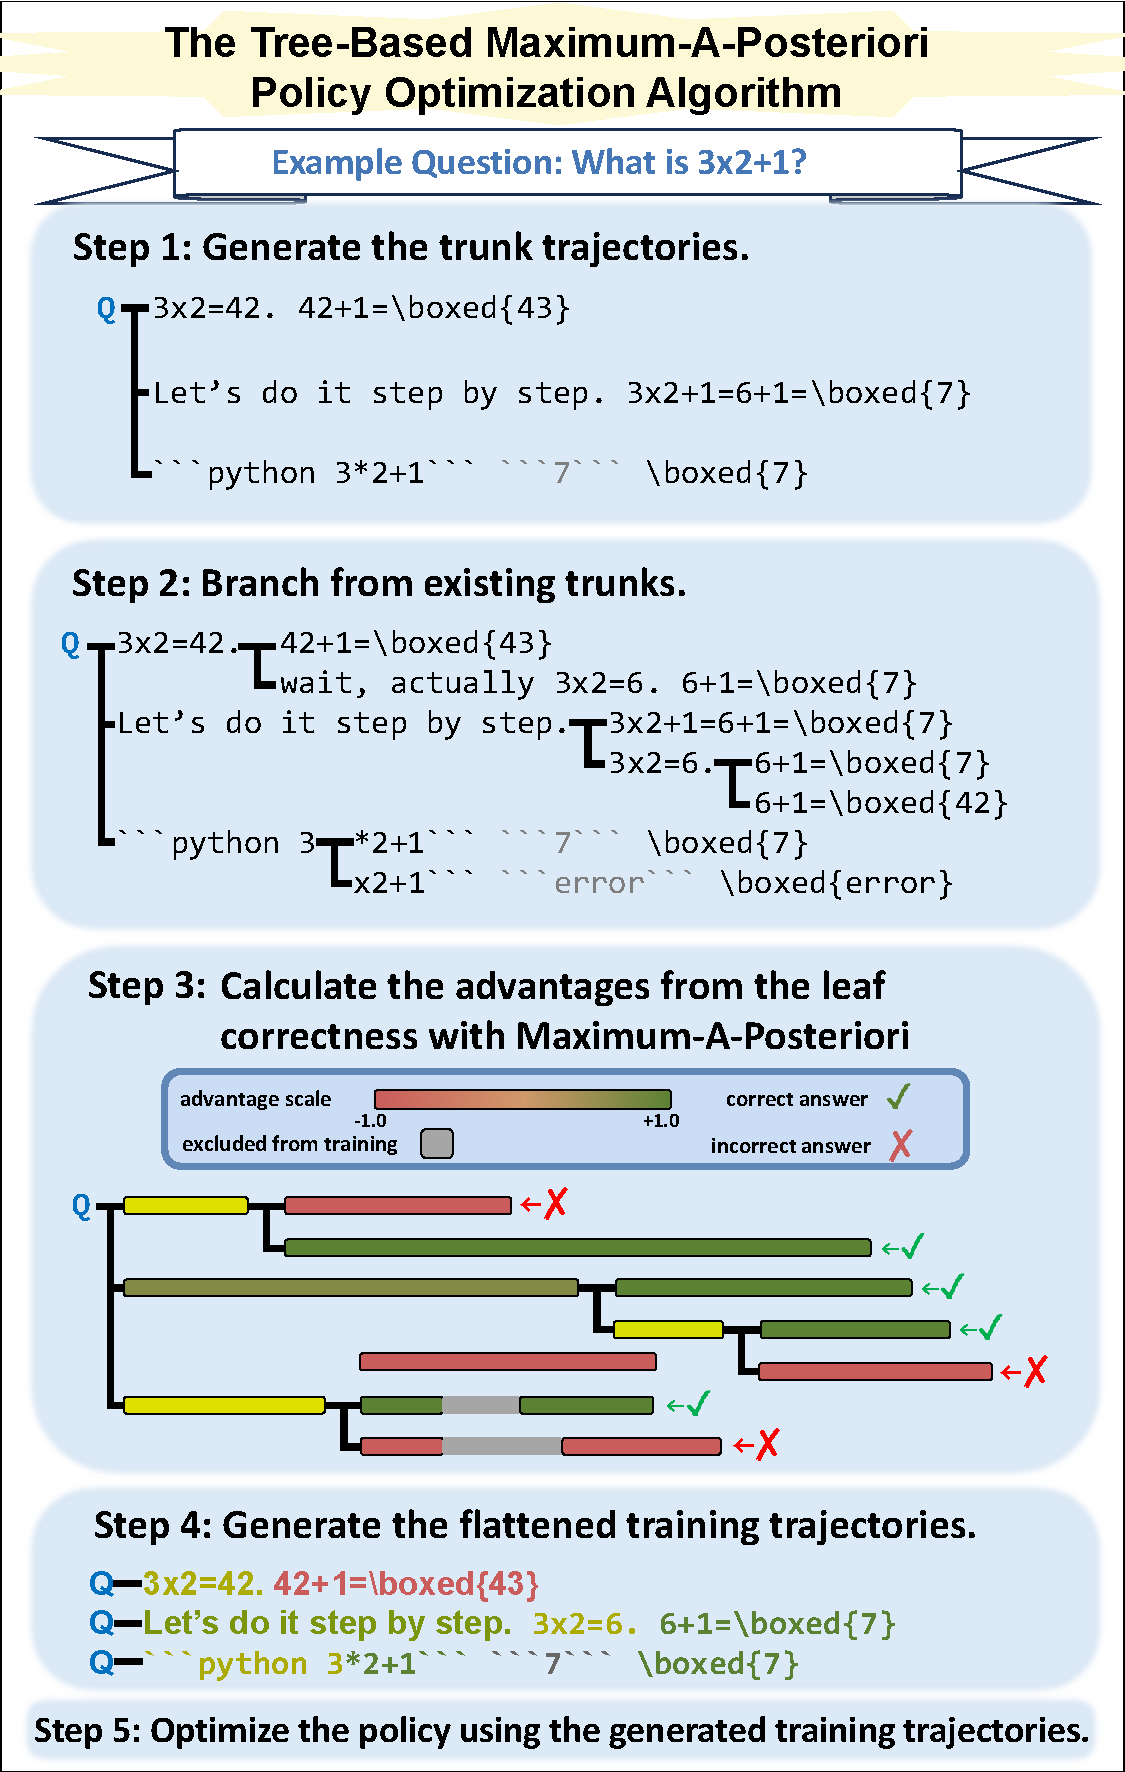
\includegraphics[width=0.49\textwidth]{images/tree_mappo_methodology.pdf}
\caption{Method overview. \ours\ samples base-policy trajectories, expands selected token-level branch points, infers segment-level contribution and uncertainty from leaf correctness, and converts the resulting posterior estimates into token-level advantages for adapter training.}
\label{fig:methodology}
\end{figure}

\section{Related Work}
\paragraph{Trajectory-level RL for reasoning.}
Reinforcement learning with verifiable rewards is a standard recipe for mathematical reasoning because final-answer correctness can often be checked automatically. PPO stabilizes policy updates with a clipped surrogate and learned value function \cite{ppo17}, while GRPO removes the critic by normalizing outcome rewards across sampled responses \cite{deepseekmath2024}. Both still face the limitation targeted here: terminal feedback can reinforce or suppress many irrelevant tokens along with the decisive reasoning steps.

\paragraph{Process supervision and verifier-based credit.}
A complementary line densifies supervision by evaluating intermediate reasoning with human step labels, automatically constructed stepwise supervision, explicit first-error localization, implicit process rewards, or alternative process-reward aggregation rules \cite{lightman2023letsverify,mathshepherd2024,selfexplore2024,prime2025,pure2025}. These methods establish the value of process-level signal, but they introduce process evaluators or explicit error-localization/aggregation mechanisms. \ours\ instead infers local contribution from correctness variation across deliberately branched policy trajectories.

\paragraph{Tree, segment, and shared-prefix credit.}
Structured-rollout methods obtain intermediate credit from shared prefixes, flexible segments, or explicit tree search. TEMPO extracts branch-gated corrections from natural prefix trees \cite{tempo2025}; SPO estimates segment-level advantages and includes a tree variant for long traces \cite{spo2025}; TreeRL branches at high-uncertainty intermediate decisions \cite{treerl2025}; TreeRPO and TreePO use tree structure for local comparisons or subgroup-relative advantages \cite{treerpo2025,treepo2025}; and TreeAdv redistributes leaf advantages over entropy-driven rollout forests \cite{treeadv2026}.

\ours\ is closest to this family, but its differentiating claim is not tree construction alone. It combines model-plausible token-level counterfactual interventions with a joint MAP estimator over latent signed segment contributions and uncertainty, rather than relying on incidental prefix overlap, Monte Carlo segment differences, entropy-only branching, empirical child-group rewards, or direct leaf-advantage redistribution.

Several of these systems report larger gains than ours under their own full training stacks; Table~\ref{tab:related-reported-results} summarizes representative numbers and why they are not directly comparable. We do not include full SPO-tree or TreePO reproductions because their methods are coupled to segment-synchronous rollout schedulers, fallback/replay rules, and objective-specific masking or subgroup normalization, rather than being drop-in replacements for our branching or advantage modules.

\paragraph{Prefix-aware and off-policy tree supervision.}
Tree-OPO \cite{treeopo2025} uses teacher-generated MCTS prefixes and staged advantage estimation to create prefix-aware off-policy training groups. By contrast, \ours\ constructs its trees from behavior-policy rollouts and is reference-policy-free: it does not require a reference policy, offline teacher trees, reward models, or process-level supervision. Our split-pipeline experiments reuse these rollouts across optimization epochs, so the training phase is not fully online or strictly on-policy after the adapter changes.

\paragraph{Fine-grained credit without explicit trees.}
Tree structure is not the only route to critic-free fine-grained credit: GRPO-$\lambda$, OAR, and OPPO localize credit using eligibility-style signals, outcome-sensitivity attribution, or Bayesian value recursion within flat or individually scored trajectories \cite{grpolambda2025,oar2026,oppo2026}. \ours\ instead actively generates local counterfactual continuations and infers shared segment contributions from descendant outcomes.

\paragraph{Agentic RL and branching granularity.}
Long-horizon agents create delayed credit-assignment challenges. GiGPO uses repeated anchor states for local agent-action comparisons \cite{gigpo2025}, and APPO argues that influential tool-agent decisions are not confined to coarse workflow stages \cite{appo2026}. \ours\ creates local comparisons at token-level reasoning prefixes rather than relying on repeated environment states or procedure-level advantage scaling.

\paragraph{Tool-augmented mathematical reasoning and benchmarks.}
Our tool setting builds on work showing that language models can interleave reasoning with program execution or external actions \cite{gao2022pal,chen2022pot,yao2022react,schick2023toolformer}. Evaluation uses mathematical reasoning resources including MATH and DeepMath-103K, with additional held-out datasets to test transfer beyond the training distribution \cite{hendrycks2021math,he2025deepmath103k}.

\begin{figure}[t]
\centering
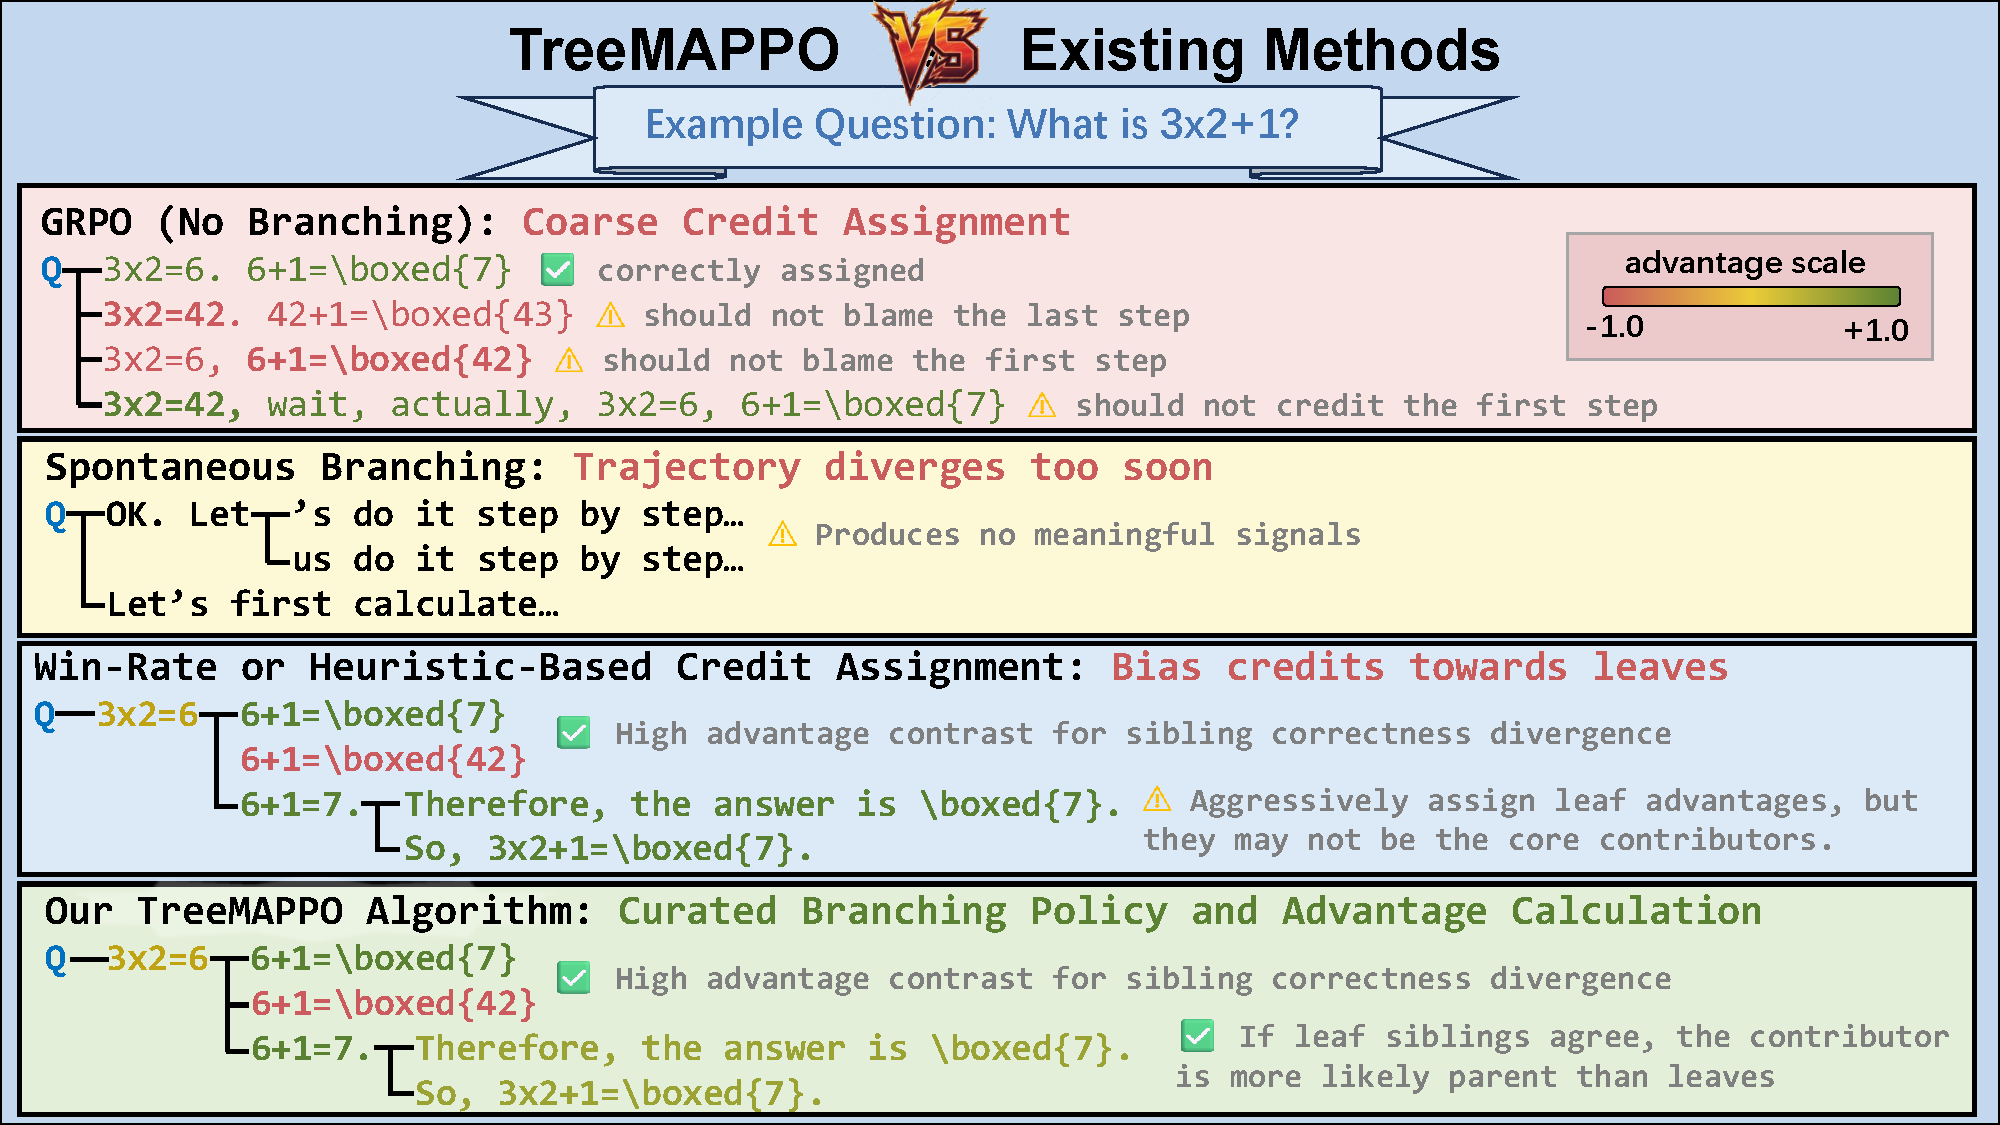
\includegraphics[width=\textwidth]{images/tree_mappo_comparison.pdf}
\caption{Comparison of credit-assignment structures. Trajectory-level GRPO assigns one normalized outcome signal to every token; TEMPO extracts branch-gated corrections from natural shared prefixes; TreeRPO uses fixed-step tree sampling and empirical child-group rewards; \ours\ combines guided token-level branching with posterior segment-credit inference.}
\label{fig:method-comparison}
\end{figure}



\section{Problem Setting and Agent Protocol}
We study question-answering agents for mathematical reasoning. Each sample provides a problem statement and a ground-truth final answer used only for post hoc correctness judgment. During rollout, the model may produce plain-text reasoning and, when enabled, invoke a Python executor.

The main methodological question is how to assign credit inside the resulting mixed text--tool trajectory after only a terminal answer judgment is observed. Our experiments keep the prompting and execution protocol fixed across training-data collection and evaluation so that differences across methods are attributable to branching and credit assignment rather than prompt format changes. Appendix~\ref{app:implementation-protocol} gives the exact tool-calling and rollout protocol.

\section{Method}
\subsection{Overview}
For each question, we first sample a set of complete trunk trajectories. We then expand a rollout tree by branching from selected token positions. Each completed leaf trajectory is judged as correct or incorrect using its extracted final boxed answer. The resulting leaf labels provide supervision for segment-level posterior inference. Posterior estimates are transformed into training advantages for model optimization, while branch selection in the split implementation uses rollout structure and model-side token statistics.

\subsection{Trajectory Tree Construction}
Branching is token-level rather than step-level. A new branch can be created in two ways:
\begin{itemize}
    \item \textbf{Segment split:} split an existing reasoning segment at an internal token position and regenerate from that point.
    \item \textbf{Node expansion:} branch again from an existing branching node, increasing its branching factor.
\end{itemize}

Each branch preserves the prefix before the selected token position and then creates a new continuation from that point. This construction makes a tree node correspond to an actual intervention in the model's decoded trajectory rather than to a manually annotated reasoning step. Appendix~\ref{app:implementation-protocol} reports the concrete branch budgets and decoding settings used in experiments.
Appendix Table~\ref{tab:guided-branching-pseudocode} gives implementation-aligned pseudocode for guided branch construction.

\subsection{MAP Credit Assignment Model}
Let $\ell$ index judged leaves and let $i$ index non-prompt segments. For each leaf $\ell$:
\begin{itemize}
    \item $y_\ell \in \{+1,-1\}$ is the correctness label.
    \item $x_{\ell,i} \in \{0,1\}$ indicates whether segment $i$ lies on the path to leaf $\ell$.
    \item Segment $i$ has mean contribution $m_i$ and log standard deviation $u_i$.
\end{itemize}

Leaf-level moments are
\begin{align}
\mu_\ell &= \sum_i x_{\ell,i} m_i, \\
\tau_\ell &= \sqrt{\sum_i x_{\ell,i} \exp(2u_i) + \varepsilon}, \\
z_\ell &= y_\ell \mu_\ell / \tau_\ell.
\end{align}
We use a probit likelihood,
\begin{equation}
p(y_\ell \mid \{m_i,u_i\}) = \Phi(z_\ell),
\end{equation}
where $\Phi$ is the standard normal CDF.

Our implementation initializes prior means at zero and optimizes the negative log posterior
\begin{equation}
\mathcal{J} = -\sum_\ell \log \Phi(z_\ell)
+ \frac{1}{2\sigma_m^2}\sum_i m_i^2
+ \frac{1}{2\sigma_u^2}\sum_i u_i^2.
\end{equation}

Optimization is performed with gradient steps and backtracking line search, together with a numerically stable implementation of $\log \Phi$ for large negative margins. Concrete prior scales, iteration counts, and numerical clamps are reported in Appendix~\ref{app:implementation-protocol}.

\subsection{Guided Token-Level Branching}
The split-pipeline implementation chooses branch points before leaf judgments are available. Branching therefore relies on rollout structure and model-side token statistics rather than posterior uncertainty. For each candidate token position, the branch score multiplies:
\begin{enumerate}
    \item a structural penalty, and
    \item the relative probability of the best alternative token that differs from the already-sampled continuation.
\end{enumerate}
Candidates whose best alternative has relative probability below $0.1$ are discarded.

For node expansion, the structural penalty is an exponential branching-factor penalty,
\begin{equation}
\gamma_{\text{node}}(b) = \exp\big(-k_{\text{node}}(b-1)\big),
\end{equation}
with $k_{\text{node}}=0.35$ in the reported experiments.
For segment splitting, the structural penalty increases with the shorter side of the split relative to average trunk length, discouraging very short fragments.

After a branch point and alternative token are selected, the current guided-branching implementation forces that selected token to be the first token of the new branch continuation. This makes the token-level branch explicit rather than merely restarting generation from the shared prefix and hoping that sampling chooses the intended alternative. We keep the non-forced version as an ablation, but use the forced-token version as the default because it better matches the intended token-level intervention.

\subsection{From Posterior Scores to Training Advantages}
After tree construction, each non-root segment receives a signed posterior score $m_i / \exp(u_i)$, where $m_i$ is the inferred mean contribution and $\exp(u_i)$ is the inferred standard deviation. The implementation then applies the same deterministic conversion chain used in the reported runs: divide by a clamped reasoning-token segment length, standardize scores within the tree, set a score to zero if mean subtraction would flip its sign, divide each shared segment score by the number of leaf trajectories that contain it, balance the total positive and negative advantage mass over the generated training set, and finally clip token-level advantages to $[-3,3]$ before optimization. The generated training samples attach these token-level advantage values aligned with the input sequence.
Appendix Table~\ref{tab:map-optimization-pseudocode} gives pseudocode for the MAP optimization and advantage conversion used by the generation phase.

The downstream training code consumes aligned token sequences, supervised target tokens, attention masks, token-level advantages, and old token log probabilities. The loss is a clipped policy-ratio surrogate over supervised positions,
\begin{equation}
\mathcal{L}_{\text{train}} = -\frac{1}{|\mathcal{S}|}
\sum_{t \in \mathcal{S}}
\min\left(
\rho_t \tilde{A}_t,
\operatorname{clip}(\rho_t,1-\epsilon,1+\epsilon)\tilde{A}_t
\right),
\end{equation}
where $\mathcal{S}$ denotes supervised token positions, $\rho_t$ is the ratio between the current token probability and the stored old token probability, and $\tilde{A}_t$ is the token advantage clipped to $[-3,3]$. This is the implemented optimization interface for injecting segment-level credit into model updates while avoiding the unbounded negative-advantage objective that arises from direct advantage-weighted cross entropy.

\subsection{Training-Set Construction}
Because many tree leaves share prefixes, naively flattening all leaves would duplicate the same segment-level credit across descendant trajectories. We therefore preserve all informative leaves while normalizing the credit assigned to shared segments.
\begin{enumerate}
    \item Discard trees whose leaves are uniformly correct or uniformly incorrect, since they provide no contrastive signal for segment-level credit.
    \item Compute segment advantages from the chosen credit estimator after leaf judgments are attached.
    \item For each segment, count how many completed leaf trajectories contain it and divide that segment's advantage by this count.
    \item Emit each remaining leaf trajectory with token-level advantages inherited from its segments, so shared prefixes contribute a fixed total amount of training signal rather than being multiplied by the number of descendants.
    \item Aggregate emitted trajectories across questions under the fixed ordering used by the training pipeline.
\end{enumerate}

Selected trajectories are then emitted under a fixed batching convention so sibling positive and negative samples from the same problem are consumed consecutively; this ordering is an implementation detail rather than an experimental variable.

\section{Baselines and Ablations}
We compare against the base model and a GRPO-style baseline with multiple complete rollouts but no token-level branching. Ablations independently vary exploration and credit estimation: TEMPO-style branching uses spontaneous shared-prefix divergence; TreeRPO-style credit replaces MAP inference with child-group outcome comparisons; TreeRL-style branching uses entropy-based branch selection; and TreeRL-style credit uses a local--global value-difference estimator. This disentangles the source of alternative trajectories from the method used to assign credit.

\section{Experimental Setup}
We evaluate \ours\ and matched baselines on Qwen2.5-7B, Qwen3-4B, Gemma-3-4B, Mistral-7B, and Llama-3.1, treating tool-enabled and no-tool settings separately. Training and validation use DeepMath, MATH, and NuminaMath; held-out testing adds AMC2023, GaoKao Math 2024, and CollegeMath. We report pass@1 accuracy as an equal-weight macro average over datasets.

The primary experiments use a split one-shot protocol: rollouts are collected from the base policy, advantage-weighted training data are generated once, and LoRA adapters are trained for multiple epochs before checkpoint validation. This differs from fully online RL, where each policy update would trigger fresh rollouts from the latest checkpoint. The split protocol is less expensive, easier to audit, and better suited to controlled comparisons under limited queue and GPU budgets; it primarily tests the quality of the generated credit-assignment data rather than full closed-loop policy-improvement dynamics.

To reduce compute-budget confounds, GRPO and tree conditions are matched by pre-filter rollout budget. In our pipeline, inference-time rollout dominates wall-clock and GPU allocation: generating multiple long reasoning trajectories is substantially more expensive than adapter updates on the resulting filtered training set. Moreover, filtering intentionally removes many zero-signal cases, especially questions whose leaves are uniformly correct or uniformly incorrect. We therefore model the primary computation budget as the number of trajectories generated before filtering. In the main 8-leaf GRPO versus 16-leaf tree comparison, GRPO receives twice as many raw questions per epoch so both settings target the same number of generated leaf trajectories before correctness filtering. This does not guarantee identical effective update mass after all-correct/all-incorrect filtering, shared-segment advantage normalization, and advantage clipping; it instead matches the dominant inference-rollout cost. Appendix~\ref{app:implementation-protocol} gives dataset construction, chunk sizes, timing audits, hyperparameters, validation cadence, and an advantage-scale audit.


\section{Results}
We report results across all completed experimental conditions. Training rollouts use $T=0.7$; all validation and held-out test rollouts are decoded greedily ($T=0$) with one trajectory per question. Intervals over ``trials'' quantify run-to-run variability of the inference and judging pipeline, not policy sampling variance, and not variance over independently seeded training runs. All held-out test rows in the main tables use five rollout trials and all six test datasets; held-out validation rows use six trials. We emphasize conservative conclusions: the evidence supports modest and repeatable validation improvements, but the broader held-out tests show that these gains do not always transfer uniformly.

\subsection{Validation Accuracy Trends}
Held-out validation shows that both GRPO and \ours\ can extract signal from the split pipeline, although gains are modest and non-monotonic across epochs. Qwen3-4B has the strongest tool-use improvements, while Gemma and Mistral highlight substantial model-family sensitivity. Full validation inventories and the central Qwen2.5-7B no-tool trend are deferred to Appendix~\ref{app:validation-inventory}.

\subsection{Held-Out Tests}
Table~\ref{tab:heldout-serious} reports held-out tests on the broader six-dataset mixture. Each row uses the best checkpoint selected by validation for that method and setting, then evaluates it with five rollout trials when per-trial results are available. The macro average gives equal weight to datasets rather than to individual examples. Checkpoint selection and evaluation coverage are reported separately in Table~\ref{tab:test-checkpoints}.

\begin{table}[t]
\centering
\resizebox{\columnwidth}{!}{%
\begin{tabular}{llccc}
\hline
Model and condition & Base & GRPO & \ours & Main observation \\
\hline
Qwen2.5-7B no-tool & \best{0.6366} & 0.6353 & 0.6304 & Validation gains do not transfer. \\
Qwen2.5-7B + tool & 0.5742 & \best{0.5850} & 0.5836 & Both trained methods improve over base. \\
Qwen3-4B no-tool & 0.6940 & \best{0.6999} & 0.6997 & Both methods improve modestly. \\
Qwen3-4B + tool & 0.6266 & 0.6487 & \best{0.6694} & \ours gives the strongest gain. \\
Gemma-3-4B no-tool & 0.5819 & 0.5802 & \best{0.5906} & \ours is positive but small. \\
Mistral-7B no-tool & 0.1636 & \best{0.1674} & 0.1567 & Mistral remains unstable. \\
Llama-3.1 no-tool & 0.3930 & 0.4115 & \best{0.4167} & Both methods improve over base. \\
\hline
\end{tabular}%
}
\caption{Main held-out test macro accuracies. Full per-dataset accuracies, confidence intervals, selected checkpoints, and evaluation coverage are reported in Appendix~\ref{app:heldout-test-details}. Bold entries mark the best macro accuracy in each model-condition block.}
\label{tab:heldout-serious}
\end{table}

The held-out tests sharpen the qualitative picture. In no-tool Qwen2.5-7B, validation gains do not reliably transfer to the broader six-dataset macro average. In tool-enabled Qwen2.5-7B, both trained methods improve over base by about one point, with \ours\ close to GRPO. Qwen3-4B is the strongest positive setting: both methods improve in no-tool testing, and \ours\ substantially outperforms GRPO in the tool setting. Gemma and Llama provide additional positive evidence for \ours\ over their base models, while Mistral remains unstable under this training recipe.

\subsection{Ablation Study}
We organize mechanism analysis into two categories. The first category consists of ablations that are compatible with our algorithmic framework and can be implemented by changing one localized component, making them useful for isolating the effect of individual mechanisms rather than reproducing an entire external system. These ablations separate branching policy from credit estimation: the TEMPO-style condition changes the branch source to spontaneous shared-prefix divergence; the TreeRPO-style condition changes only the segment-credit estimator to child-group win-rate comparison; and the two TreeRL-style conditions separately test entropy-guided branching and local--global value-difference credit. Guided-branching experiments use forced selected branch tokens by default; non-forced branching is retained only as a mechanism ablation.

\begin{table}[t]
\centering
\resizebox{\textwidth}{!}{%
\begin{tabular}{lcccccc}
\hline
Qwen2.5-7B no-tool variant & Best val. epoch & Val. base & Best val. & Val. gain & Test epoch & Test macro \\
\hline
GRPO baseline & 30 & \acc{0.6468}{0.0033} & \best{\acc{0.6538}{0.0021}} & +0.0069 & 30 & \best{\acc{0.6353}{0.0118}} \\
\ours, non-forced token & 20 & \acc{0.6399}{0.0026} & \acc{0.6472}{0.0018} & +0.0072 & 20 & \acc{0.6294}{0.0085} \\
\ours, forced token & 50 & \acc{0.6436}{0.0025} & \acc{0.6523}{0.0016} & +0.0087 & 50 & \acc{0.6304}{0.0081} \\
TEMPO-style branching & 70 & \acc{0.6418}{0.0032} & \acc{0.6515}{0.0020} & \best{+0.0097} & 70 & \acc{0.6326}{0.0144} \\
TreeRPO-style credit & 40 & \acc{0.6426}{0.0027} & \acc{0.6519}{0.0018} & +0.0094 & 40 & \acc{0.6272}{0.0054} \\
TreeRL-style branching & 20 & \acc{0.6402}{0.0045} & \acc{0.6480}{0.0041} & +0.0078 & 20 & \acc{0.6195}{0.0069} \\
TreeRL-style credit & 60 & \best{\acc{0.6474}{0.0044}} & \acc{0.6528}{0.0014} & +0.0054 & 60 & \acc{0.6334}{0.0062} \\
TreeRL combined & 40 & \acc{0.6449}{0.0032} & \acc{0.6507}{0.0024} & +0.0058 & 40 & \acc{0.6341}{0.0110} \\
Branch budget 8 & 10 & \acc{0.6446}{0.0040} & \acc{0.6471}{0.0031} & +0.0025 & 10 & \acc{0.6274}{0.0076} \\
Branch budget 32 & 60 & \acc{0.6428}{0.0026} & \acc{0.6503}{0.0041} & +0.0075 & 60 & \acc{0.6333}{0.0105} \\
\hline
\end{tabular}
}
\caption{Qwen2.5-7B no-tool ablations. Validation numbers are held-out macro averages with 95\% confidence intervals from six rollout trials; testing uses five trials and six datasets. Gain is the difference between the best validation checkpoint and the same run's epoch-0 validation score. Bold underlined entries mark the largest value in each numeric column.}
\label{tab:ablation-results}
\end{table}

Table~\ref{tab:ablation-results} shows that most tree-structured variants improve on their own validation baselines, but the strongest validation gain does not automatically yield the strongest broad test result. TEMPO-style branching has the largest validation gain, suggesting that natural prefix diversity already exposes useful alternatives in this no-tool setting. TreeRPO-style credit is close in validation but weaker on the six-dataset test, indicating that coarse child-group outcome comparisons can overfit the validation distribution. The TreeRL-style credit and combined variants have comparatively strong held-out test macro averages, while entropy-only branching is weaker, suggesting that credit estimation is at least as important as branch-location selection. The forced-token mechanism improves validation over the non-forced version, motivating the default intervention design, although this advantage does not consistently transfer to the held-out test suite.

The second category consists of closely related systems whose core mechanisms are either orthogonal to \ours\ or too tightly coupled to their own training stacks to reproduce within our framework without major infrastructure changes. For SPO-tree, TreePO, TreeAdv, APPO, GRPO-$\lambda$, OAR, and LamPO, a same-hyperparameter replication would not isolate a single shared mechanism and would be dominated by differences in online rollout scheduling, evaluator design, objective details, or training scale. We therefore report their working principles and claimed improvements as coarse context in Appendix Table~\ref{tab:related-reported-results}, rather than treating them as directly comparable baselines.

\subsection{Stability Diagnostics}
Several completed runs are negative results that shape our conclusions. They indicate that the method is sensitive to optimizer aggressiveness, adapter configuration, and model family, motivating the conservative settings used in the main tables. Appendix~\ref{app:stability-diagnostics} summarizes the concrete failed and unstable settings.

The branch-budget sensitivity study is deferred to Appendix~\ref{app:branch-budget}: increasing the branch budget from 8 to 32 improves the held-out test macro average slightly, but the effect is not monotonic enough to be a primary claim.

\subsection{Tool-Use Case Study}
A representative Qwen2.5-7B tool-enabled \ours\ trajectory illustrates the type of error--repair structure that segment-level credit can distinguish. The model first sets up the right equation and calls Python, but writes an incorrect answer before reading the tool result; after the tool returns $9$, the later segment repairs the answer, producing $\boxed{9}$ as the final response. \ours\ assigns weak negative credit to the flawed pre-tool span and positive credit to the post-tool repair, with segment advantages $-0.114,+0.222,+0.635,+0.635,+0.576$. The complete colored trajectory and prompts are shown in Appendix~\ref{app:case-study-details}.

\section{Discussion}
The results point to a trade-off among credit granularity, rollout budget, and optimization stability. GRPO is inexpensive and stable because it assigns one group-normalized terminal signal to full responses, but this simplicity can blur late repairs and intermediate mistakes. Tree-based methods spend more inference budget to expose local alternatives and then train on variable segment-level advantages; this helps when the tree contains meaningful correctness contrasts, but can introduce higher-variance updates when branches fragment unimportant regions or the model family is adapter-sensitive.

This also connects to recent observations that saturated reasoning data can be ``too correct to learn'' \cite{cuts2026}. In our setting, only mixed-correctness trees provide informative contrast for segment-level credit: if all leaves for a question are correct or all are incorrect, the tree contains little supervised evidence about which local segment caused success or failure. Appendix Table~\ref{tab:mixed-correctness-efficiency} shows that only 36--53\% of TreeMAPPO training-rollout questions yield mixed-correctness trees in the reported settings. This partially explains why reference-policy-free RL from terminal correctness is difficult and why the overall improvements remain modest when many questions produce uniform outcomes.

Tool use appears to make segmented credit more valuable. Tool trajectories can contain error--feedback--repair transitions, where early reasoning is harmful but later tool-informed reasoning is helpful. This is consistent with the case study and the strongest Qwen3 tool result favoring \ours, and motivates analyzing tool-enabled settings separately from no-tool reasoning.

The ablation results should therefore be read as a method-characteristic map rather than a single global ranking. Spontaneous or entropy-based branching can work when models naturally produce diverse alternatives, while guided token branching is more useful when plausible but under-sampled decisions matter. Win-rate and local--global backups can be competitive when correctness changes align with large subtree boundaries, whereas the MAP estimator is better matched to cases where several shared segments jointly explain mixed descendants.

Several implementation choices follow from this interpretation. Branch selection currently relies on structural penalties and alternative-token probability rather than posterior uncertainty, because judgments are produced after tree construction in the split pipeline. The training loss uses a clipped policy-ratio surrogate with token-level advantages, keeping the optimization interface close to standard policy-gradient practice while preserving tree-based credit assignment. The forced-token branch variant is the default because the branch score evaluates a specific alternative token, so forcing that token makes the generated intervention match the scored decision.

\section{Limitations and Future Work}
TreeMAPPO incurs additional rollout cost and is evaluated primarily in a split one-shot rather than fully online training regime. Gains are modest and transfer unevenly across models and datasets, motivating larger-scale online experiments, stronger optimizer controls, and repeated independent seeds. The MAP estimator also assumes additive segment contributions and relies on final-answer extraction, assumptions that may become restrictive in more complex agentic environments. Finally, our ablations approximate several related tree-credit ideas within a common rollout and training infrastructure, but they are not full reproductions of SPO-tree or TreePO. Those methods couple their credit estimators to segment-synchronous tree generation, replay or fallback rules, and probability-mask or subgroup-normalized objectives \cite{spo2025,treepo2025}; reproducing them faithfully would require a separate pipeline rather than only swapping the branching or advantage module.

\section{Conclusion}
We presented \ours, a trajectory-tree method for fine-grained credit assignment in agentic LLM training. The core idea is to branch reasoning trajectories at token granularity, infer segment-level contribution from mixed-success descendants, and convert those estimates into training signals for subsequent optimization. Completed split-pipeline experiments show that \ours\ can outperform baseline methods under some configurations, especially when the foundation model and tool-calling context create recoverable intermediate mistakes. The results also reveal a trade-off among finer credit assignment, additional rollout budget, and training stability on trajectories with variable advantages. We therefore view \ours\ not as a uniformly dominant replacement for GRPO, but as a worthwhile option to try as training scale and computation budget increase, particularly for agentic settings where tool feedback can turn early mistakes into later corrections.

\subsection*{AI use statement}
Generative AI tools were used to assist with code implementation, experiment orchestration, log inspection, result aggregation, and manuscript editing. All reported results, claims, code changes, and paper text were reviewed by the authors, who take responsibility for the final content of this work.

\subsection*{Ethics statement}
This work studies mathematical reasoning benchmarks and does not involve human-subject data collection. The main ethical risks are ordinary risks of improving automated reasoning agents, including possible misuse and over-reliance on generated reasoning traces. We mitigate these risks by evaluating only answer correctness on public mathematical datasets and by reporting negative and mixed results alongside positive findings.

\subsection*{Reproducibility statement}
The paper reports the model families, rollout protocol, training hyperparameters, validation cadence, and testing protocol used in the experiments. The implementation keeps explicit judging/scoring passes and concise run summaries for validation and testing so that experiment outputs can be audited and regenerated.



\bibliography{references}
\bibliographystyle{iclr2027_conference}

\appendix
\section{Implementation and Protocol Details}
\label{app:implementation-protocol}

\paragraph{Tool-calling protocol.}
Each prompt contains the problem statement and, when tool use is enabled, a specification that Python can be called by emitting a fenced markdown block. The model may interleave reasoning and tool use. When a fenced Python block closes, generation pauses, the tool executes, and the tool response is appended to the context. The model is instructed to present its final answer in \texttt{\textbackslash boxed\{\}}. If generation reaches a control handoff without a boxed answer, the framework requests continuation until a boxed answer is produced or rollout termination conditions are hit.

\paragraph{Rollout and tree hyperparameters.}
In the default configuration for the main tool-using setup, each tree begins with 4 trunk trajectories and expands to 16 total trajectories. Branch-budget ablations use 8 and 32 total trajectories. We keep a fixed decoding temperature within each tree; in the reported configurations, this value is $T=0.7$ for trunk generation, continuation, and branch expansion.

\paragraph{Rollout-budget balancing.}
For the main chunked comparison, GRPO uses 8 complete leaf trajectories per question, while the tree setting uses 16 leaf trajectories per question. Because rollout inference is the bottleneck, we approximately equalize rollout work per training epoch by assigning GRPO twice as many raw questions per chunk: 250 questions for GRPO and 125 questions for tree rollouts. Thus both settings target 2{,}000 generated leaf trajectories per epoch before correctness filtering. Direct run checks confirm this layout for the Qwen2.5 no-tool run: the first GRPO chunk contains question indices 0--249 with 8 leaves per question, and the first tree chunk contains question indices 0--124 with 16 leaves per question, giving 2{,}000 leaves in both chunks. The first-run timing summaries are also comparable for Qwen2.5: 235 seconds per GRPO no-tool chunk versus 207 seconds per tree no-tool chunk, and 237 seconds per GRPO tool chunk versus 210 seconds per tree tool chunk. After judging and filtering, the number of accepted training trajectories can differ because all-correct and all-incorrect questions are removed. This is expected rather than a failure of the budget model: those removed samples carry no contrastive credit signal, and the scarce resource being controlled is the cost of generating candidate trajectories, not the final number of supervised token updates.

\begin{table*}[t]
\centering
\small
\setlength{\tabcolsep}{3pt}
\resizebox{\textwidth}{!}{%
\begin{tabular}{llrrrrrrr}
\hline
Model & Setting & Questions & All correct & All incorrect & Mixed & Filtered & Train traj. & Traj./question \\
\hline
Qwen2.5-7B & No-tool & 8{,}750 & 3{,}883 (44.4\%) & 1{,}431 (16.4\%) & 3{,}436 (39.3\%) & 60.7\% & 54{,}976 & 6.3 \\
Qwen2.5-7B & Tool & 8{,}750 & 3{,}228 (36.9\%) & 1{,}496 (17.1\%) & 4{,}026 (46.0\%) & 54.0\% & 64{,}416 & 7.4 \\
Qwen3-4B & No-tool & 6{,}250 & 3{,}120 (49.9\%) & 847 (13.6\%) & 2{,}283 (36.5\%) & 63.5\% & 36{,}528 & 5.8 \\
Qwen3-4B & Tool & 6{,}250 & 2{,}637 (42.2\%) & 934 (14.9\%) & 2{,}679 (42.9\%) & 57.1\% & 42{,}864 & 6.9 \\
Gemma-3-4B & No-tool & 6{,}250 & 2{,}421 (38.7\%) & 1{,}526 (24.4\%) & 2{,}303 (36.8\%) & 63.2\% & 36{,}848 & 5.9 \\
Mistral-7B & No-tool & 6{,}250 & 149 (2.4\%) & 3{,}112 (49.8\%) & 2{,}989 (47.8\%) & 52.2\% & 47{,}824 & 7.7 \\
Llama-3.1 & No-tool & 6{,}250 & 1{,}112 (17.8\%) & 1{,}843 (29.5\%) & 3{,}295 (52.7\%) & 47.3\% & 52{,}720 & 8.4 \\
\hline
\end{tabular}
}
\caption{Training-rollout correctness breakdown for TreeMAPPO generation runs. ``Filtered'' is the share of questions with all-correct or all-incorrect leaves, which produce no within-question contrastive credit signal and are removed before training trajectory construction. ``Train traj.'' counts accepted leaf trajectories after this question-level filtering.}
\label{tab:mixed-correctness-efficiency}
\end{table*}

Table~\ref{tab:mixed-correctness-efficiency} shows that rollout efficiency varies substantially by model family and tool setting. For Qwen2.5-7B and Qwen3-4B, enabling tools reduces the all-correct fraction and increases the mixed-correctness fraction by roughly 6--7 points, consistent with tool feedback creating more recoverable error--repair variation. Across no-tool models, stronger or more saturated models such as Qwen3-4B produce many all-correct trees, while weaker models such as Mistral produce many all-incorrect trees. Llama has the highest mixed-correctness rate in this table, indicating many informative rollouts, but the main results show that informative contrast alone is insufficient without stable optimization and good transfer.

\begin{table}[t]
\centering
\small
\begin{tabular}{lrrrr}
\hline
Method & Questions & Train traj. & Mean $|\bar{A}|$ & Median $|\bar{A}|$ \\
\hline
GRPO & 17{,}500 & 53{,}200 & 0.825 & 0.577 \\
\ours & 8{,}750 & 54{,}976 & 0.355 & 0.281 \\
\hline
\end{tabular}
\caption{Training-set advantage-scale audit for Qwen2.5-7B no-tool runs. $|\bar{A}|$ is the absolute average token advantage for an emitted leaf trajectory, as recorded by the generation statistics after shared-segment normalization and token clipping but before final positive/negative mass balancing. The lower mean for \ours\ reflects shared-segment advantage normalization across descendant leaves rather than weaker rollout correctness alone.}
\label{tab:qwen25-notool-advantage-scale}
\end{table}

\paragraph{MAP-credit optimization details.}
The hyperparameter configuration uses $\sigma_m = 1.0$, $\sigma_u = 1.0$, $\varepsilon = 10^{-6}$, 120 optimization iterations, and log-standard-deviation clamps in $[-4,2]$. These settings are fixed across the main TreeMAPPO comparisons unless an ablation explicitly changes the credit-estimation rule.

\paragraph{Datasets.}
Training and validation are built from DeepMath, MATH, and NuminaMath. The training split contains 5{,}000 samples per dataset, interleaved across the three in-distribution datasets. The validation split contains 1{,}000 validation samples per dataset drawn from disjoint index ranges after the training slice. The held-out test split aggregates DeepMath, MATH, NuminaMath, AMC2023, GaoKao Math 2024, and CollegeMath. For datasets with more than 1{,}000 test rows, 1{,}000 are sampled with seed 42; for DeepMath, which lacks a dedicated test split in the evaluation pipeline, evaluation rows are drawn from the training split after clearing the reserved training and validation examples.

\paragraph{Training and evaluation protocol.}
The main stable runs use chunked one-shot training, where each epoch consumes one generated training chunk and recovery restarts at whole-chunk boundaries. Primary experiments use LoRA rank 32 and learning rate $10^{-6}$, with Adam state and learning-rate warmup enabled unless stated otherwise. Held-out validation is run at epoch 0 and then every 10 epochs for long runs, with multiple validation rollout trials used to reduce sampling noise. We use LoRA-based fine-tuning for the primary experiments; full-model training is deferred because queueing and memory costs are substantially higher.

\section{Full Validation Inventory}
\label{app:validation-inventory}
Table~\ref{tab:validation-results} gives the full held-out validation inventory used for checkpoint selection and trend analysis.

\begin{figure}[t]
\centering
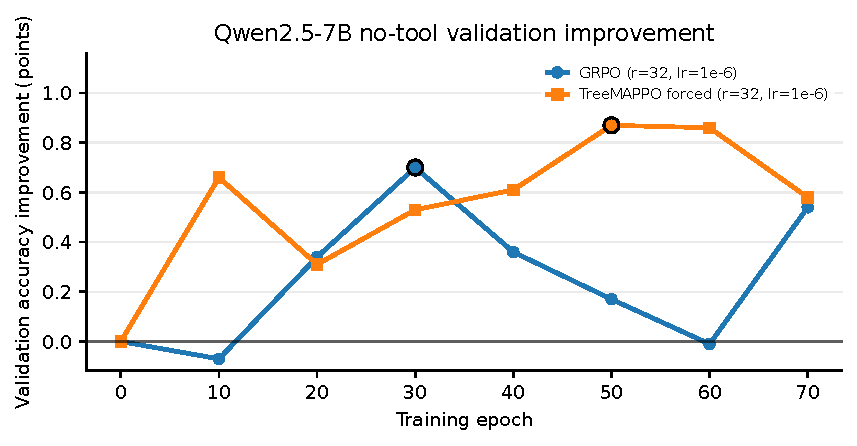
\includegraphics[width=\columnwidth]{images/qwen25_notool_epoch_improvement.pdf}
\caption{Validation accuracy improvement over the base checkpoint for Qwen2.5-7B in the no-tool setting. Both lines use LoRA rank 32 and learning rate $10^{-6}$; the y-axis reports percentage-point change relative to each method's epoch-0 validation accuracy.}
\label{fig:qwen25-notool-improvement}
\end{figure}

\begin{table}[t]
\centering
\resizebox{\textwidth}{!}{%
\begin{tabular}{llccccccc}
\hline
Model and condition & Method & Trials & Epochs audited & Base & Best epoch & Best & Gain & Last \\
\hline
Qwen2.5-7B no-tool & GRPO & 6 & 0,10,\ldots,70 & \best{\acc{0.6468}{0.0033}} & 30 & \best{\acc{0.6538}{0.0021}} & +0.0069 & \best{\acc{0.6522}{0.0039}} \\
Qwen2.5-7B no-tool & \ours & 6 & 0,10,\ldots,70 & \acc{0.6436}{0.0025} & 50 & \acc{0.6523}{0.0016} & \best{+0.0087} & \acc{0.6494}{0.0035} \\
\hline
Qwen2.5-7B + tool & GRPO & 6 & 0,10,\ldots,70 & \best{\acc{0.6142}{0.0033}} & 30 & \best{\acc{0.6246}{0.0024}} & \best{+0.0104} & \acc{0.6171}{0.0046} \\
Qwen2.5-7B + tool & \ours & 6 & 0,10,\ldots,70 & \acc{0.6134}{0.0034} & 50 & \acc{0.6236}{0.0033} & +0.0101 & \best{\acc{0.6181}{0.0016}} \\
\hline
Qwen3-4B no-tool & GRPO & 6 & 0,10,\ldots,50 & \best{\acc{0.6901}{0.0021}} & 50 & \best{\acc{0.6991}{0.0038}} & \best{+0.0089} & \best{\acc{0.6991}{0.0038}} \\
Qwen3-4B no-tool & \ours & 6 & 0,10,\ldots,50 & \acc{0.6894}{0.0017} & 30 & \acc{0.6944}{0.0024} & +0.0050 & \acc{0.6849}{0.0047} \\
\hline
Qwen3-4B + tool & GRPO & 6 & 0,10,\ldots,50 & \best{\acc{0.6446}{0.0030}} & 40 & \best{\acc{0.6617}{0.0046}} & \best{+0.0172} & \acc{0.6521}{0.0044} \\
Qwen3-4B + tool & \ours & 6 & 0,10,\ldots,50 & \acc{0.6434}{0.0034} & 50 & \acc{0.6605}{0.0023} & +0.0171 & \best{\acc{0.6605}{0.0023}} \\
\hline
Gemma-3-4B no-tool & GRPO & 6 & 0,10,\ldots,50 & \best{\acc{0.5640}{0.0022}} & 50 & \best{\acc{0.5647}{0.0032}} & +0.0007 & \best{\acc{0.5647}{0.0032}} \\
Gemma-3-4B no-tool & \ours & 6 & 0,10,\ldots,50 & \acc{0.5621}{0.0030} & 40 & \acc{0.5643}{0.0029} & \best{+0.0023} & \acc{0.5594}{0.0034} \\
\hline
Mistral-7B no-tool & GRPO & 6 & 0,10,\ldots,50 & \best{\acc{0.1747}{0.0043}} & 40 & \acc{0.1802}{0.0013} & +0.0055 & \acc{0.1729}{0.0021} \\
Mistral-7B no-tool & \ours & 6 & 0,10,\ldots,50 & \acc{0.1747}{0.0019} & 10 & \best{\acc{0.1819}{0.0031}} & \best{+0.0072} & \best{\acc{0.1788}{0.0023}} \\
\hline
Llama-3.1 no-tool & GRPO & 6 & 0,10,\ldots,50 & \acc{0.4415}{0.0038} & 30 & \best{\acc{0.4684}{0.0018}} & \best{+0.0269} & \best{\acc{0.4609}{0.0064}} \\
Llama-3.1 no-tool & \ours & 6 & 0,10,\ldots,50 & \best{\acc{0.4454}{0.0035}} & 40 & \acc{0.4589}{0.0029} & +0.0135 & \acc{0.4568}{0.0053} \\
\hline
\end{tabular}%
}
\caption{Audited held-out validation results. Values are pass@1 macro averages on the validation mixture, reported as mean with 95\% confidence interval over rollout trials. All rows use six validation trials and epochs that are 0 or multiples of 10. Bold underlined entries mark the largest value within each model-condition comparison block.}
\label{tab:validation-results}
\end{table}

\section{Stability and Negative-Run Diagnostics}
\label{app:stability-diagnostics}
Several failed or unhelpful runs influenced the final experiment design. Qwen2.5-7B \ours\ at LoRA rank 32 with learning rate $5\times10^{-5}$ collapsed in earlier validation, while the same rank with learning rate $10^{-6}$ remained stable. SGD/no-warmup variants did not show useful trends and were removed from the main schedule. Mistral remains difficult under this recipe: its absolute accuracy is low, and \ours\ is below the base model on held-out testing despite a small validation gain. These outcomes motivate treating adapter rank, learning rate, optimizer state, and model-family sensitivity as substantive empirical factors rather than incidental implementation details.

\section{Full Held-Out Test Details}
\label{app:heldout-test-details}
Table~\ref{tab:heldout-serious-details} reports the per-dataset held-out test results that underlie the compact main-text table.

\begin{table}[t]
\centering
\resizebox{\textwidth}{!}{%
\begin{tabular}{llccccccc}
\hline
& & \multicolumn{3}{c}{In-distribution datasets} & \multicolumn{3}{c}{Out-of-distribution datasets} & \\
\cline{3-5}\cline{6-8}
Model and condition & Method & DeepMath & MATH & NuminaMath & AMC 2023 & GaoKao 2024 & CollegeMath & Macro avg. \\
\hline
Qwen2.5-7B no-tool & Base & \acc{0.6034}{0.0030} & \best{\acc{0.7400}{0.0056}} & \best{\acc{0.6160}{0.0211}} & \acc{0.5400}{0.0480} & \acc{0.6000}{0.0511} & \best{\acc{0.7204}{0.0029}} & \best{\acc{0.6366}{0.0145}} \\
Qwen2.5-7B no-tool & GRPO & \acc{0.5886}{0.0028} & \acc{0.7338}{0.0056} & \acc{0.5940}{0.0133} & \acc{0.5200}{0.0475} & \best{\acc{0.6692}{0.0185}} & \acc{0.7062}{0.0042} & \acc{0.6353}{0.0118} \\
Qwen2.5-7B no-tool & \ours & \best{\acc{0.6050}{0.0059}} & \acc{0.7362}{0.0031} & \acc{0.5880}{0.0073} & \best{\acc{0.5900}{0.0480}} & \acc{0.5615}{0.0185} & \acc{0.7016}{0.0043} & \acc{0.6304}{0.0081} \\
\hline
Qwen2.5-7B + tool & Base & \acc{0.5806}{0.0042} & \acc{0.6812}{0.0042} & \acc{0.5540}{0.0048} & \acc{0.4650}{0.0720} & \acc{0.5154}{0.0511} & \acc{0.6488}{0.0082} & \acc{0.5742}{0.0118} \\
Qwen2.5-7B + tool & GRPO & \acc{0.5806}{0.0063} & \acc{0.6988}{0.0053} & \acc{0.5660}{0.0100} & \best{\acc{0.4750}{0.0410}} & \best{\acc{0.5385}{0.0413}} & \acc{0.6514}{0.0041} & \best{\acc{0.5850}{0.0149}} \\
Qwen2.5-7B + tool & \ours & \best{\acc{0.5840}{0.0060}} & \best{\acc{0.7036}{0.0046}} & \best{\acc{0.5780}{0.0243}} & \acc{0.4600}{0.0504} & \acc{0.5231}{0.0185} & \best{\acc{0.6530}{0.0028}} & \acc{0.5836}{0.0116} \\
\hline
Qwen3-4B no-tool & Base & \acc{0.6716}{0.0035} & \acc{0.8244}{0.0032} & \acc{0.6240}{0.0202} & \acc{0.5800}{0.0392} & \acc{0.7615}{0.0282} & \acc{0.7022}{0.0022} & \acc{0.6940}{0.0109} \\
Qwen3-4B no-tool & GRPO & \best{\acc{0.6846}{0.0038}} & \acc{0.8250}{0.0069} & \best{\acc{0.6340}{0.0078}} & \best{\acc{0.6250}{0.0219}} & \acc{0.7231}{0.0369} & \best{\acc{0.7078}{0.0042}} & \best{\acc{0.6999}{0.0037}} \\
\hspace{0pt}Qwen3-4B no-tool & \ours & \acc{0.6840}{0.0092} & \best{\acc{0.8368}{0.0047}} & \acc{0.6120}{0.0073} & \acc{0.5850}{0.0250} & \best{\acc{0.7769}{0.0554}} & \acc{0.7034}{0.0022} & \acc{0.6997}{0.0098} \\
\hline
Qwen3-4B + tool & Base & \acc{0.6078}{0.0056} & \acc{0.7458}{0.0044} & \acc{0.5900}{0.0164} & \acc{0.5850}{0.0250} & \acc{0.5692}{0.0440} & \acc{0.6616}{0.0029} & \acc{0.6266}{0.0099} \\
Qwen3-4B + tool & GRPO & \acc{0.6288}{0.0063} & \best{\acc{0.7734}{0.0073}} & \acc{0.5480}{0.0144} & \best{\acc{0.6650}{0.0250}} & \acc{0.6077}{0.0369} & \acc{0.6692}{0.0069} & \acc{0.6487}{0.0084} \\
Qwen3-4B + tool & \ours & \best{\acc{0.6340}{0.0095}} & \acc{0.7670}{0.0021} & \best{\acc{0.6020}{0.0096}} & \acc{0.6500}{0.0410} & \best{\acc{0.6846}{0.0282}} & \best{\acc{0.6788}{0.0035}} & \best{\acc{0.6694}{0.0101}} \\
\hline
Gemma-3-4B no-tool & Base & \acc{0.4780}{0.0067} & \acc{0.7606}{0.0043} & \acc{0.5580}{0.0114} & \acc{0.4800}{0.0646} & \acc{0.5692}{0.0282} & \best{\acc{0.6456}{0.0049}} & \acc{0.5819}{0.0115} \\
Gemma-3-4B no-tool & GRPO & \acc{0.4810}{0.0059} & \acc{0.7610}{0.0027} & \best{\acc{0.5920}{0.0114}} & \acc{0.4300}{0.0240} & \acc{0.5769}{0.0238} & \acc{0.6402}{0.0039} & \acc{0.5802}{0.0093} \\
Gemma-3-4B no-tool & \ours & \best{\acc{0.4846}{0.0122}} & \best{\acc{0.7670}{0.0078}} & \acc{0.5720}{0.0130} & \best{\acc{0.5050}{0.0567}} & \best{\acc{0.5769}{0.0238}} & \acc{0.6382}{0.0047} & \best{\acc{0.5906}{0.0117}} \\
\hline
Mistral-7B no-tool & Base & \acc{0.1910}{0.0092} & \acc{0.1474}{0.0035} & \acc{0.1900}{0.0124} & \best{\acc{0.0650}{0.0332}} & \best{\acc{0.2154}{0.0452}} & \acc{0.1728}{0.0040} & \acc{0.1636}{0.0129} \\
Mistral-7B no-tool & GRPO & \best{\acc{0.2136}{0.0062}} & \acc{0.1528}{0.0063} & \best{\acc{0.2560}{0.0237}} & \acc{0.0500}{0.0155} & \acc{0.1538}{0.0238} & \best{\acc{0.1782}{0.0069}} & \best{\acc{0.1674}{0.0031}} \\
Mistral-7B no-tool & \ours & \acc{0.2014}{0.0058} & \best{\acc{0.1562}{0.0061}} & \acc{0.1980}{0.0180} & \acc{0.0350}{0.0250} & \acc{0.1769}{0.0511} & \acc{0.1728}{0.0032} & \acc{0.1567}{0.0097} \\
\hline
Llama-3.1 no-tool & Base & \acc{0.3250}{0.0065} & \acc{0.4954}{0.0032} & \acc{0.4040}{0.0100} & \acc{0.2850}{0.0332} & \acc{0.3846}{0.0238} & \acc{0.4642}{0.0052} & \acc{0.3930}{0.0036} \\
Llama-3.1 no-tool & GRPO & \best{\acc{0.3666}{0.0111}} & \best{\acc{0.5168}{0.0071}} & \acc{0.4340}{0.0159} & \acc{0.2750}{0.0268} & \best{\acc{0.4077}{0.0452}} & \acc{0.4688}{0.0051} & \acc{0.4115}{0.0086} \\
Llama-3.1 no-tool & \ours & \acc{0.3314}{0.0045} & \acc{0.5146}{0.0118} & \best{\acc{0.4480}{0.0114}} & \best{\acc{0.3200}{0.0098}} & \best{\acc{0.4077}{0.0612}} & \best{\acc{0.4784}{0.0080}} & \best{\acc{0.4167}{0.0081}} \\
\hline
\end{tabular}%
}
\caption{Held-out test results by dataset. Values are pass@1 accuracies with 95\% confidence intervals from per-trial scores. Bold underlined entries mark the largest value within each model-condition comparison block. Table~\ref{tab:forced-token-results} separately compares forced and non-forced TreeMAPPO variants.}
\label{tab:heldout-serious-details}
\end{table}

\section{Checkpoint and Mechanism Tables}
Table~\ref{tab:test-checkpoints} records which checkpoints and evaluations support the held-out test table in the main text. Table~\ref{tab:forced-token-results} provides the forced-token mechanism comparison summarized in the main results.

\begin{table}[t]
\centering
\resizebox{\textwidth}{!}{%
\begin{tabular}{llccc}
\hline
Model and condition & Method & Selected epoch & Testing trials & Dataset coverage \\
\hline
Qwen2.5-7B no-tool & Base & 0 & 5 & 6/6 \\
Qwen2.5-7B no-tool & GRPO & 30 & 5 & 6/6 \\
Qwen2.5-7B no-tool & \ours & 50 & 5 & 6/6 \\
\hline
Qwen2.5-7B + tool & Base & 0 & 5 & 6/6 \\
Qwen2.5-7B + tool & GRPO & 30 & 5 & 6/6 \\
Qwen2.5-7B + tool & \ours & 50 & 5 & 6/6 \\
\hline
Qwen3-4B no-tool & Base & 0 & 5 & 6/6 \\
Qwen3-4B no-tool & GRPO & 50 & 5 & 6/6 \\
Qwen3-4B no-tool & \ours & 30 & 5 & 6/6 \\
\hline
Qwen3-4B + tool & Base & 0 & 5 & 6/6 \\
Qwen3-4B + tool & GRPO & 40 & 5 & 6/6 \\
Qwen3-4B + tool & \ours & 50 & 5 & 6/6 \\
\hline
Gemma-3-4B no-tool & Base & 0 & 5 & 6/6 \\
Gemma-3-4B no-tool & GRPO & 50 & 5 & 6/6 \\
Gemma-3-4B no-tool & \ours & 40 & 5 & 6/6 \\
\hline
Mistral-7B no-tool & Base & 0 & 5 & 6/6 \\
Mistral-7B no-tool & GRPO & 40 & 5 & 6/6 \\
Mistral-7B no-tool & \ours & 20 & 5 & 6/6 \\
\hline
Llama-3.1 no-tool & Base & 0 & 5 & 6/6 \\
Llama-3.1 no-tool & GRPO & 30 & 5 & 6/6 \\
Llama-3.1 no-tool & \ours & 40 & 5 & 6/6 \\
\hline
\end{tabular}%
}
\caption{Checkpoint-selection and evaluation-coverage table for the held-out tests in Table~\ref{tab:heldout-serious}. All listed rows use per-trial, per-dataset results under the unified judging and scoring pipeline.}
\label{tab:test-checkpoints}
\end{table}

\begin{table}[t]
\centering
\resizebox{\textwidth}{!}{%
\begin{tabular}{llcccc}
\hline
Condition & Variant & Best val. epoch & Best val. & Test epoch & Test macro \\
\hline
Qwen2.5-7B no-tool & Non-forced token & 20 & \acc{0.6472}{0.0018} & 20 & \acc{0.6294}{0.0085} \\
Qwen2.5-7B no-tool & Forced token & 50 & \best{\acc{0.6523}{0.0016}} & 50 & \best{\acc{0.6304}{0.0081}} \\
\hline
Qwen2.5-7B + tool & Non-forced token & 70 & \acc{0.6193}{0.0047} & 70 & \best{\acc{0.5962}{0.0044}} \\
Qwen2.5-7B + tool & Forced token & 50 & \best{\acc{0.6236}{0.0033}} & 50 & \acc{0.5836}{0.0116} \\
\hline
\end{tabular}%
}
\caption{Forced-token mechanism ablation for TreeMAPPO. Forced-token branching improves the selected validation checkpoint in both Qwen2.5-7B settings, but the held-out test difference is small and reverses in the tool setting.}
\label{tab:forced-token-results}
\end{table}

\section{Branching-Budget Sensitivity}
\label{app:branch-budget}
Our experimental plan includes 8-, 16-, and 32-trajectory variants for the Qwen2.5-7B no-tool setting. The held-out tests do not show a simple monotonic scaling law. Branch budget 32 has a higher held-out test macro average than branch budget 8, but the gap is small and remains within the scale of other run-to-run differences.

\begin{figure}[t]
\centering
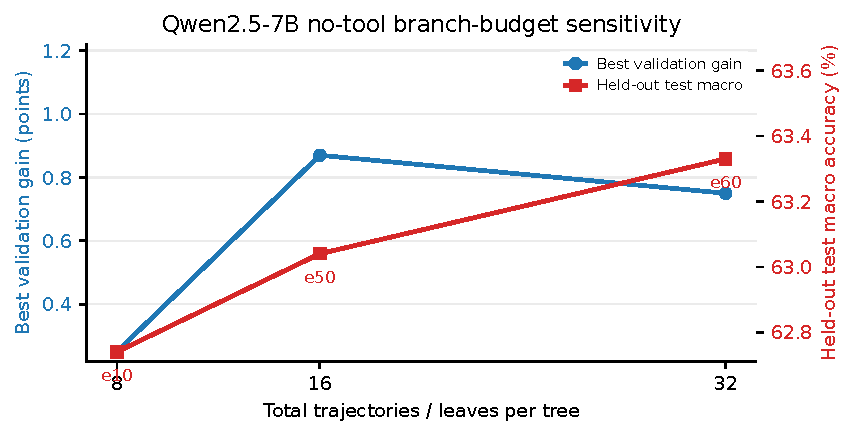
\includegraphics[width=\columnwidth]{images/qwen25_branch_budget_sensitivity.pdf}
\caption{Branching-budget sensitivity for Qwen2.5-7B no-tool TreeMAPPO variants. The validation line reports the best validation improvement over each run's epoch-0 checkpoint; the held-out test line reports the five-trial, six-dataset macro accuracy at the validation-selected checkpoint.}
\label{fig:branch-budget}
\end{figure}

\section{Reported Results from Closely Related Systems}
\label{app:related-reported-results}
Table~\ref{tab:related-reported-results} summarizes representative improvements reported by closely related fine-grained, tree-based, or group-relative RL systems. We remove implementation-specific caveats from the table itself and state the key qualification here: these results are not directly comparable to our split-pipeline LoRA experiments because they differ in computation budget, training scale, online versus split rollout policy, majority-vote or pass@1 evaluation, datasets, and whether reference trajectories, process signals, or specialized rollout systems are used.

\begin{table*}[t]
\centering
\scriptsize
\setlength{\tabcolsep}{4pt}
\resizebox{\textwidth}{!}{%
\begin{tabular}{p{0.13\textwidth}p{0.34\textwidth}p{0.44\textwidth}}
\hline
Method & Main mechanism & Reported improvement in its paper \\
\hline
SPO / SPO-tree \cite{spo2025} & Flexible segment partition, MC segment values, tree-based segment reuse, probability-mask optimization & SPO-chain reports \textbf{6--12 point} gains over PPO/GRPO on GSM8K; SPO-tree reports \textbf{7--11 point} gains over GRPO on MATH500 under 2K/4K context evaluation. \\
TreeRPO \cite{treerpo2025} & Tree sampling with step/group relative reward expectations & Reports Qwen2.5-Math average Pass@1 increasing from \textbf{19.0\% to 35.5\%}, plus \textbf{2.9 points} over GRPO and \textbf{18.1\%} shorter responses. \\
TreePO \cite{treepo2025} & Segment-synchronous tree rollout with dynamic branching/fallback and subgroup-relative advantages & Reports GRPO with TreePO sampling improving overall major@16 accuracy from \textbf{46.63\% to 54.61\%}; TreePO advantage adds \textbf{2.27--3.6 points} while reducing sampling GPU hours by \textbf{12--43\%}. \\
TEMPO \cite{tempo2025} & Prefix-to-tree conversion of naturally sampled responses with branch-gated TD corrections & Reports higher validation and final performance than PPO/GRPO on Qwen3-1.7B/4B across math and medical QA, with roughly matched wall-clock time. \\
TreeAdv \cite{treeadv2026} & Entropy-driven rollout forests with token-level redistribution of leaf advantages & Reports consistent gains over GRPO/GSPO across \textbf{10 math benchmarks} while using substantially fewer generated tokens under matched supervision/data/decoding budgets. \\
TreeRL \cite{treerl2025} & On-policy tree search with value backup from subtree outcomes & Reports improved trajectory diversity and optimization signals relative to independent multi-chain sampling. \\
APPO \cite{appo2026} & Fine-grained agentic branching score plus procedure-level advantage scaling & Reports nearly \textbf{4-point} improvement over strong agentic RL baselines on \textbf{13 benchmarks} with efficient tool calls. \\
GRPO-$\lambda$ \cite{grpolambda2025} & Critic-free eligibility-style credit assignment over sequence log-probabilities & Reports \textbf{30--40\%} improved training performance curves and more than \textbf{3 points} average gain over GRPO, including a \textbf{4.5-point} gain for a 7B model. \\
OAR \cite{oar2026} & Outcome-sensitivity reshaping by perturbation or gradient proxy & Reports significant gains over strong GRPO baselines, with gradient-based OAR-G approaching perturbation-based OAR-P at low overhead. \\
LamPO \cite{lampo2026} & Pairwise decomposed group advantages with confidence-aware weighting & Reports consistent gains over GRPO and recent RLVR variants on AIME, MATH-500, and GPQA-Diamond. \\
\hline
\end{tabular}
}
\caption{Representative reported improvements from closely related fine-grained, tree-based, or group-relative RL methods. Bold text highlights the numerical gains reported by the corresponding papers. The values are not directly comparable to our results because computation budget, training scale, evaluation policy, datasets, and supervision assumptions differ.}
\label{tab:related-reported-results}
\end{table*}

\section{Implementation-Aligned Pseudocode}
\label{app:pseudocode}
Tables~\ref{tab:guided-branching-pseudocode} and~\ref{tab:map-optimization-pseudocode} summarize the two implementation paths most relevant for reimplementation. The pseudocode follows the split pipeline used in the experiments: tree rollout produces unjudged trees, a separate judging pass attaches leaf correctness, and training-set generation computes advantages only after judging.

\begin{table*}[t]
\centering
\fbox{\begin{minipage}{0.94\textwidth}
\small
\textbf{Input:} question $q$, rollout config $(T,L)$, decoding temperature, force-selected-token flag.\\
\textbf{Output:} rollout tree with prompt/root segment, generated reasoning/tool segments, leaf answers, and no correctness labels.
\begin{enumerate}
    \item Initialize a tree with the prompt segment for $q$ as the root.
    \item While fewer than $T$ trunk leaves exist, generate a complete response from the root prompt and attach the response as a new trunk leaf.
    \item While fewer than $L$ total leaves exist:
    \begin{enumerate}
        \item Enumerate existing reasoning tokens. Prompt tokens and tool-response tokens are not candidate branch points.
        \item For the first reasoning token of a segment, treat the candidate as node expansion. Exclude first tokens already used by sibling branches. Choose the highest-probability remaining top-$k$ token if its probability relative to the original top token is at least $0.1$.
        \item For an internal reasoning token, treat the candidate as a segment split. Exclude the token that was actually generated at that position. Choose the highest-probability remaining top-$k$ token if its relative probability is at least $0.1$.
        \item Score each node-expansion candidate by alternative-token relative probability times a branching-factor penalty. Score each segment-split candidate by alternative-token relative probability times a segment-length penalty. Entropy replaces relative probability only in the TreeRL-style branching ablation.
        \item Select the positive-score candidate with maximum score. If no such candidate exists, stop expanding the tree.
        \item If the candidate is a segment split, split the selected segment before the selected token; if it is node expansion, branch from the selected node.
        \item If forced branching is enabled, append the selected alternative token to the generation prompt, generate the remaining continuation, and then record that selected token and its stored log probability as the first token of the new branch.
        \item Attach the generated continuation and update the tree status.
    \end{enumerate}
    \item Return the tree artifact. Leaf correctness is intentionally absent and is added only by the judging pass.
\end{enumerate}
\end{minipage}}
\caption{Guided token-level tree construction. This matches the current split-pipeline implementation: branch selection uses model-side top-$k$ token statistics and structural penalties, not posterior uncertainty from leaf judgments.}
\label{tab:guided-branching-pseudocode}
\end{table*}

\begin{table*}[t]
\centering
\fbox{\begin{minipage}{0.94\textwidth}
\small
\textbf{Input:} judged tree with segment set $\mathcal{S}$, leaf labels $y_\ell\in\{+1,-1\}$, and leaf-to-root segment paths.\\
\textbf{Output:} token-level training trajectories with old log probabilities and clipped advantages.
\begin{enumerate}
    \item Discard the root prompt segment from posterior variables. For every non-root segment $i$, initialize mean $m_i=0$ and log standard deviation $u_i=0$.
    \item For every judged leaf $\ell$, build its path indicator $x_{\ell,i}$ over non-root segments.
    \item Minimize the negative log posterior
    \[
    \sum_i \frac{(m_i-0)^2}{2\sigma_m^2}
    + \sum_i \frac{u_i^2}{2\sigma_u^2}
    - \sum_\ell \log \Phi\!\left(
        \frac{y_\ell \sum_i x_{\ell,i}m_i}
        {\sqrt{\sum_i x_{\ell,i}\exp(2u_i)+\varepsilon}}
    \right),
    \]
    using gradient descent with backtracking line search for at most 120 iterations.
    \item Clamp every $u_i$ to $[-4,2]$ after each candidate update.
    \item Convert posteriors to raw segment scores by $m_i/\exp(u_i)$, divide by a clamped reasoning-token segment length, then normalize scores across segments by subtracting the segment-score mean and dividing by the segment-score standard deviation. If mean subtraction would flip a segment's sign, set that normalized segment score to zero.
    \item Keep only mixed-correctness questions for training-set generation. All-correct and all-incorrect trees provide no contrastive segment-credit signal and are filtered out.
    \item Divide each segment score by the number of leaf trajectories that contain that segment so shared-prefix credit is not duplicated across leaves.
    \item For each selected leaf trajectory, assign the segment score to generated reasoning/tool-call tokens, assign zero and ignored labels to prompt/tool-response tokens, and retain old token log probabilities from rollout.
    \item Balance positive and negative advantage mass across the emitted training set unless a positive-only ablation is explicitly requested, then clip final token advantages to the configured range.
\end{enumerate}
\end{minipage}}
\caption{MAP segment-credit optimization and conversion to token-level training data. This table describes the default \ours\ advantage path; TreeRPO, TreeRL, and GRPO ablations replace only the segment-advantage calculation step.}
\label{tab:map-optimization-pseudocode}
\end{table*}

\section{Qualitative Case Study Details}
\label{app:case-study-details}
We inspected generated training trajectories for a Qwen2.5-7B tool-enabled \ours\ run and selected a NuminaMath question that also appears in the no-tool ablation results: ``A woman is 42 years of age and her daughter is 8 years old. In a certain number of years, the mother will be three times as old as her daughter. How many years will it take for the mother to be three times as old as her daughter?'' The correct equation is $42+x=3(8+x)$, giving $x=9$.

Figure~\ref{fig:case-study-prompts} gives the exact prompts seen by the model in the tool and no-tool \ours\ settings, including the Qwen chat-template markers. Figures~\ref{fig:case-study-trajectory} and~\ref{fig:case-study-ablation-trajectories} show exact raw trajectory excerpts from \ours\ and available ablations. For the main tool/no-tool comparison, we use the same question. For the ablation panels, we intentionally allow different questions because questions whose sampled leaves are uniformly correct or uniformly incorrect produce zero or near-zero advantages under several credit rules; such cases are uninformative for visualizing how each method distributes credit. The displayed ablation questions are listed in each panel.

The colors are used only to visualize token-level training advantages for readers and automated reviewers; they are not part of the model input or output. Prompt tokens and Python tool outputs have ignored labels and are not colored. Each trajectory uses an adaptive muted red--yellow--green interpolation: the largest absolute advantage in that trajectory saturates to dark red or dark green, so color shows within-trajectory credit structure while the printed numbers show cross-trajectory scale. In the tool-enabled \ours\ trajectory, the model first solves the equation with a Python call but writes an incorrect answer, receives the actual tool response $9$, and then corrects the final answer by emitting $\boxed{9}$ in the final response. The early setup receives weak negative credit, while the post-tool repair receives positive credit.

\begin{figure*}[t]
\centering
\fbox{\begin{minipage}{0.95\textwidth}
\small
\textbf{Question.} A woman is 42 years old and her daughter is 8 years old. In how many years will the mother be three times as old as her daughter?\\[2pt]
\textbf{Colored raw trajectory excerpt.}
\begingroup\ttfamily\scriptsize\raggedright\sloppy
\textcolor[RGB]{142,106,41}{Let's denote the number of years from now when the mother will be three times as old as her daughter by \textbackslash{}( x \textbackslash{}). Currently, the mother is 42 years old and the daughter is 8 years old. In \textbackslash{}( x \textbackslash{}) years, the ages are \textbackslash{}(42+x\textbackslash{}) and \textbackslash{}(8+x\textbackslash{}). According to the problem,}
\textcolor[RGB]{101,120,49}{ the mother's age will be three times the daughter's age: \textbackslash{}[42+x=3(8+x)\textbackslash{}]. Now we solve this equation using Python: ```python from sympy import symbols, Eq, solve ... solution}
\textcolor[RGB]{20,110,55}{[0] ``` :boxed\{6\}. So, it will take 6 years for the mother to be three times as old as her daughter.}\\
<tool\_response>9</tool\_response>\\
\textcolor[RGB]{20,110,55}{It seems there was an error in my previous calculation. Let's re-solve the equation step by step: \textbackslash{}[42+x=3(8+x)\textbackslash{}], so \textbackslash{}[42+x=24+3x\textbackslash{}].}
\textcolor[RGB]{32,111,54}{ Rearranging terms, \textbackslash{}[42-24=3x-x\textbackslash{}], \textbackslash{}[18=2x\textbackslash{}], and \textbackslash{}[x=9\textbackslash{}]. Therefore, the correct answer is \textbackslash{}[\textbackslash{}boxed\{9\}\textbackslash{}].}
\endgroup\\[2pt]
\textbf{Observed segment advantages.} $-0.114,\,+0.222,\,+0.635,\,+0.635,\,+0.576$.
\end{minipage}}
\caption{Qwen2.5-7B tool-use case study. The black tool-response line is ignored by the training loss but explains why the following model segment can repair the answer.}
\label{fig:case-study-trajectory}
\end{figure*}

\begin{figure*}[t]
\centering
\fbox{\begin{minipage}{0.47\textwidth}
\small
\textbf{Tool prompt, exact decoded trajectory prefix.}\\[2pt]
\begingroup\ttfamily\scriptsize\raggedright\sloppy
<|im\_start|>system\\
You are Qwen, created by Alibaba Cloud. You are a helpful assistant.<|im\_end|>\\
<|im\_start|>user\\
You are a helpful agent that solves the following problem.\\
Question: A woman is 42 years of age and her daughter is 8 years old. In a certain number of years, the mother will be three times as old as her daughter. How many years will it take for the mother to be three times as old as her daughter?\\
You are encouraged to use the Python code executor to help you do calculations to ensure correctness. You can invoke python code by emitting a Python markdown code block like this:\\
```python\\
import numpy as np\\
A = np.array([[2, 1], [1, -1]])\\
b = np.array([5, 1])\\
solution = np.linalg.solve(A, b)\\
solution\\
```\\
You should reason step by step, and put the final answer in a \textbackslash{}boxed\{\}.\\
Begin your reasoning:<|im\_end|>\\
<|im\_start|>assistant
\endgroup
\end{minipage}}
\hfill
\fbox{\begin{minipage}{0.47\textwidth}
\small
\textbf{No-tool prompt, exact decoded trajectory prefix.}\\[2pt]
\begingroup\ttfamily\scriptsize\raggedright\sloppy
<|im\_start|>system\\
You are Qwen, created by Alibaba Cloud. You are a helpful assistant.<|im\_end|>\\
<|im\_start|>user\\
You are a helpful agent that solves the following problem.\\
Question: A woman is 42 years of age and her daughter is 8 years old. In a certain number of years, the mother will be three times as old as her daughter. How many years will it take for the mother to be three times as old as her daughter?\\
You should reason step by step, and put the final answer in a \textbackslash{}boxed\{\}.\\
Begin your reasoning:<|im\_end|>\\
<|im\_start|>assistant
\endgroup
\end{minipage}}
\caption{Exact prompts for the same Qwen2.5-7B case-study question. These are the prompts used for the displayed trajectories; they are not manually rewritten prompts.}
\label{fig:case-study-prompts}
\end{figure*}

\begin{figure*}[t]
\centering
\fbox{\begin{minipage}{0.95\textwidth}
\small
\textbf{\ours, no-tool.} \emph{Question:} A woman is 42 years old and her daughter is 8 years old. In how many years will the mother be three times as old as her daughter?\\
The sampled no-tool tree solves the age equation directly, so the posterior has little corrective contrast to exploit.\\
\begingroup\ttfamily\scriptsize\raggedright\sloppy
\textcolor[RGB]{20,110,55}{Let's denote the number of years from now when the mother will be three times as old as her daughter as \textbackslash{}(x\textbackslash{}). Currently, the mother's age is 42 years and the daughter's age is 8 years. In \textbackslash{}(x\textbackslash{}) years, the mother's age will be \textbackslash{}(42+x\textbackslash{}) and the daughter's age will be \textbackslash{}(8+x\textbackslash{}).}
We can set up the equation \textbackslash{}[42+x=3(8+x)\textbackslash{}], solve it, and obtain \textbackslash{}(x=9\textbackslash{}). The final answer is \textbackslash{}(\textbackslash{}boxed\{9\}\textbackslash{}).
\endgroup\\[-2pt]
\textbf{Advantages:} $\textcolor[RGB]{20,110,55}{+0.074},0$.\\[4pt]

\textbf{GRPO, no-tool.} \emph{Question:} Find the auxiliary equation for the ordinary differential equation with constant coefficients \((x^2D^2+xD+1)y=\sin(2\log x)\sin(\log x)\).\\
GRPO assigns one terminal group-normalized advantage to the entire response.\\
\begingroup\ttfamily\scriptsize\raggedright\sloppy
\textcolor[RGB]{20,110,55}{\detokenize{To find the auxiliary equation for the given ordinary differential equation with constant coefficients, we first recognize that the equation is not in a standard constant-coefficient form because the operator contains \(x^2D^2+xD+1\). We rewrite it through the substitution \(t=\log x\), where \(xD\) acts like differentiation with respect to \(t\). This yields the auxiliary equation \(m^2+1=0\).}}
\endgroup\\[-2pt]
\textbf{Advantages:} $\textcolor[RGB]{20,110,55}{+1.732}$ for this representative response.\\[4pt]

\textbf{TEMPO-style branching.} \emph{Question:} Find the auxiliary equation for the ordinary differential equation with constant coefficients \((x^2D^2+xD+1)y=\sin(2\log x)\sin(\log x)\).\\
Spontaneous prefix-tree branching produces a nonzero but fragmented early credit pattern.\\
\begingroup\ttfamily\scriptsize\raggedright\sloppy
\textcolor[RGB]{113,121,48}{To find the auxiliary equation for the given ordinary differential equation, we need to}
\textcolor[RGB]{123,122,47}{ follow these steps.}
\textcolor[RGB]{139,81,37}{ First identify the}
\textcolor[RGB]{102,120,48}{ homogeneous part of the ODE:}
\textcolor[RGB]{20,110,55}{\detokenize{ \((x^2D^2+xD+1)y=0\). Assume \(y=x^m\), substitute \(y'=mx^{m-1}\) and \(y''=m(m-1)x^{m-2}\), and simplify to \(m^2+1=0\).}}
\endgroup\\[-2pt]
\textbf{Advantages:} $\textcolor[RGB]{113,121,48}{+0.162},\textcolor[RGB]{123,122,47}{+0.111},\textcolor[RGB]{139,81,37}{-0.263},\textcolor[RGB]{102,120,48}{+0.217},\textcolor[RGB]{20,110,55}{+0.633}$.
\end{minipage}}
\vspace{4pt}
\fbox{\begin{minipage}{0.95\textwidth}
\small
\textbf{TreeRPO-style credit.} \emph{Question:} Suppose \(g(x)=5x-3\). What is \(g^{-1}(g^{-1}(14))\)?\\
The child-group win-rate rule gives a strong sign change around the transition from generic inverse derivation to the nested evaluation.\\
\begingroup\ttfamily\scriptsize\raggedright\sloppy
\textcolor[RGB]{141,97,40}{\detokenize{To solve for \(g^{-1}(g^{-1}(14))\), first find the inverse of \(g(x)=5x-3\). Set \(y=5x-3\), solve \(x=(y+3)/5\), and obtain \(g^{-1}(x)=(x+3)/5\).}}
\textcolor[RGB]{20,110,55}{\detokenize{ Then compute \(g^{-1}(14)=17/5\), followed by \(g^{-1}(17/5)=((17/5)+3)/5=32/25\). Therefore, the final answer is \(\boxed{32/25}\).}}
\endgroup\\[-2pt]
\textbf{Advantages:} $\textcolor[RGB]{141,97,40}{-0.525},\textcolor[RGB]{20,110,55}{+2.000}$.\\[4pt]

\textbf{TreeRL-style credit.} \emph{Question:} Given \(f(x,y)=e^{-(x+y)}\) for \(x>0,y>0\), compute \(P(Y>X+1)\).\\
The local--global value rule creates a coarse negative-to-positive split over the integral setup and evaluation.\\
\begingroup\ttfamily\scriptsize\raggedright\sloppy
\textcolor[RGB]{133,43,29}{\detokenize{To compute \(P(Y>X+1)\), integrate \(e^{-(x+y)}\) over \(x>0\) and \(y>x+1\). Set up \( \int_0^\infty \int_{x+1}^\infty e^{-(x+y)}\,dy\,dx \).}}
\textcolor[RGB]{20,110,55}{\detokenize{ The inner integral becomes \( \int_{2x+1}^\infty e^{-u}\,du=e^{-(2x+1)} \), after which the remaining integral can be evaluated.}}
\endgroup\\[-2pt]
\textbf{Advantages:} $\textcolor[RGB]{133,43,29}{-0.219},\textcolor[RGB]{20,110,55}{+0.281}$.\\[4pt]

\textbf{TreeRL-style branching.} \emph{Question:} Evaluate \( \lim_{x\to0}\left(1/\tan^2x-1/x^2\right) \).\\
Entropy-guided branching yields a long recovery pattern with a negative initial transformation and a positive Taylor-expansion segment.\\
\begingroup\ttfamily\scriptsize\raggedright\sloppy
\textcolor[RGB]{139,83,37}{\detokenize{Start by writing \(\tan x=\sin x/\cos x\), so \(1/\tan^2x=\cos^2x/\sin^2x\). Combining terms gives \((x^2\cos^2x-\sin^2x)/(x^2\sin^2x)\).}}
\textcolor[RGB]{20,110,55}{\detokenize{ Then analyze the numerator and denominator as \(x\to0\) using Taylor series for \(\sin x\) and \(\cos x\), which reveals the limiting constant after cancellation.}}
\endgroup\\[-2pt]
\textbf{Advantages:} $\textcolor[RGB]{139,83,37}{-0.323},\textcolor[RGB]{20,110,55}{+0.805}$.
\end{minipage}}
\caption{Representative trajectory excerpts for available Qwen2.5-7B no-tool ablations. Unlike the main tool/no-tool comparison, ablation panels may use different questions so that the visualized examples avoid the uniform-correctness regime where several advantage rules collapse to zero. The examples are reconstructed from judged trajectories for qualitative analysis.}
\label{fig:case-study-ablation-trajectories}
\end{figure*}

This appendix is qualitative rather than a substitute for aggregate validation. It illustrates why the \ours\ design combines guided branching with posterior segment credit. GRPO supplies only a whole-response terminal signal, so it cannot distinguish setup, computation, and repair inside a response. TreeRPO- and TreeRL-style backups can create useful sign changes, but their values are coarser because they are backed up from subtree correctness rates rather than inferred as latent segment contributions. TEMPO-style branching and TreeRL-style entropy branching can expose alternative paths, but their branch construction is less tightly coupled to the token-level intervention used by \ours. In the tool-enabled \ours\ trajectory, the method preserves the mistaken pre-tool context, observes the tool response, and assigns positive credit to the later repair segment without treating the entire response as uniformly good.


\end{document}
